% 
% Annual Cognitive Science Conference
% Sample LaTeX Paper -- Proceedings Format
% 

% Original : Ashwin Ram (ashwin@cc.gatech.edu)       04/01/1994
% Modified : Johanna Moore (jmoore@cs.pitt.edu)      03/17/1995
% Modified : David Noelle (noelle@ucsd.edu)          03/15/1996
% Modified : Pat Langley (langley@cs.stanford.edu)   01/26/1997
% Latex2e corrections by Ramin Charles Nakisa        01/28/1997 
% Modified : Tina Eliassi-Rad (eliassi@cs.wisc.edu)  01/31/1998
% Modified : Trisha Yannuzzi (trisha@ircs.upenn.edu) 12/28/1999 (in process)
% Modified : Mary Ellen Foster (M.E.Foster@ed.ac.uk) 12/11/2000
% Modified : Ken Forbus                              01/23/2004
% Modified : Eli M. Silk (esilk@pitt.edu)            05/24/2005
% Modified : Niels Taatgen (taatgen@cmu.edu)         10/24/2006
% Modified : David Noelle (dnoelle@ucmerced.edu)     11/19/2014

%% Change "letterpaper" in the following line to "a4paper" if you must.

\documentclass[10pt,letterpaper]{article}

\usepackage{cogsci}
\usepackage{pslatex}
\usepackage{apacite}
\usepackage{subcaption}
\usepackage{todonotes}
\usepackage{amsmath}
\usepackage{color}
\usepackage{booktabs}
\usepackage{caption}
\captionsetup{belowskip=0pt,aboveskip=2pt}
\setlength{\textfloatsep}{8pt}

\definecolor{Green}{RGB}{10,200,100}
\newcommand{\ndg}[1]{\textcolor{Green}{[ndg: #1]}}  
\definecolor{Blue}{RGB}{10,100,200}
\newcommand{\jd}[1]{\textcolor{Blue}{[jd: #1]}} 
\definecolor{Red}{RGB}{178,34,34}
\newcommand{\mf}[1]{\textcolor{Red}{[mf: #1]}} 
\definecolor{DarkOrange}{RGB}{255,100,50}
\newcommand{\mht}[1]{\textcolor{DarkOrange}{[mht: #1]}}  


%% commands
\newcommand{\set}[1]{\left\{#1\right\}}
\DeclareMathOperator{\expo}{exp}
\newcommand{\citet}[1]{\citeA{#1}}
\newcommand{\citep}[1]{\cite{#1}}

\newcommand{\tableref}[1]{Table \ref{#1}}
\newcommand{\figref}[1]{Fig.~\ref{#1}}
\newcommand{\appref}[1]{Appendix \ref{#1}}
\newcommand{\sectionref}[1]{Section \ref{#1}}


\title{What does the crowd believe? A hierarchical approach to estimating subjective beliefs
  from empirical data}
 
\author{{\large \bf Michael Franke, Fabian Dablander, Anthea Sch\"{o}ller} \\
  \{michael.franke, fabian.dablander, anthea.schoeller\}@uni-tuebingen.de \\
  Department of Linguistics, Wilhelmstra\ss e 19 \\
  72074 T\"{u}bingen, Germany \AND
  {\large \bf Erin Bennett, Judith Degen, Michael Henry Tessler, Justine Kao, Noah D. Goodman}\\
  \{ebennett, jdegen, mtessler, justinek, ngoodman\}@stanford.edu \\
  Department of Psychology, Stanford University \\
  450 Serra Mall, Stanford, CA 94305 USA }


\begin{document}

\maketitle

\begin{abstract}
  People's beliefs about everyday events are both of theoretical interest in their own right
  and an important ingredient in model building---especially in Bayesian cognitive models of
  phenomena such as logical reasoning, future predictions, and language use. Here, we explore
  several recently used methods for measuring subjective beliefs about unidimensional
  contiguous properties, such as the likely price of a new watch. As a first step towards a way
  of assessing and comparing belief elicitation methods, we use hierarchical Bayesian modeling
  for inferring likely population-level beliefs as the central tendency of participants'
  individual-level beliefs. Three different dependent measures are considered: (i) slider
  ratings of (relative) likelihood of intervals of values, (ii) a give-a-number task, and (iii)
  choice of the more likely of two intervals of values. Our results suggest that using averaged
  normalized slider ratings for binned quantities is a practical and fairly good approximator
  of inferred population-level beliefs.

  \textbf{Keywords:} subjective beliefs, hierarchical modeling, Bayesian data analysis,
  Bayesian cognitive models
\end{abstract}




\section{Motivation}

When trying to understand observed behavior we readily ascribe beliefs and desires to fellow
agents. This happens intuitively, in folk psychology, but also in science. Scientific
ascription of latent mental states plays an important role in many explanations of higher-order
cognition: decision making, reasoning, language use, etc. It is therefore vital to have methods
for validating explanatory mental state ascriptions.

A family of models where this is particularly pressing are Bayesian models of cognition which
seek to explain task behavior in a variety of domains as partially informed by what
participants believe about mundane events---their \emph{prior beliefs}. Take interpretation of
language.  ``That watch cost a million dollars,'' tends to be interpreted as hyperbole:
conveying affect rather than literal truth.  Empirical data on whether similar statements are
understood as hyperbole can be explained well by a Bayesian model of utterance interpretation
\citep{KaoWu2014:Nonliteral-Unde}. This model assigns a crucial role to an empirical measure of
participants' expectations about the likely or normal price of a watch---only when the uttered
price is sufficiently unlikely \emph{a priori} will hyperbolic interpretation be possible.
Other examples of domains in which empirically successful models have included a measure of
participants' prior beliefs include making predictions about everyday events
\citep{GriffithsTenenbaum2006:Optimal-Predict}, referential reasoning
\citep{FrankGoodman2012:Predicting-Prag}, strength of pragmatic enrichments
\citep{DegenTessler2015:Wonky-worlds:-L}, or quantifier interpretation
\citep{SchollerFranke2015:Semantic-values}.

Many methods have been used to build prior distributions used in Bayesian cognitive models.
One method of getting at subjective beliefs is to take actual frequencies as an approximation
to subjective beliefs \cite<e.g.>{GriffithsTenenbaum2006:Optimal-Predict}. Unfortunately,
frequency data may be unavailable (e.g., one-shot events) or deviate from participants'
subjective beliefs in crucial respects.

Another common approach is to empirically measure subjective beliefs by \emph{give-a-number}
tasks. The simplest version would be this: being told that John just bought a new watch,
participants are asked for a single numerical estimate of its price. This task is easy to
comprehend and implement, but a single number does not provide much information about the
subjective belief that it is a manifestation of. One solution is to infer which parameterized
distribution best explains the observed number choices, either at the individual level
\citep{Manski2004:Measuring-Expec} or at the population level
\citep{TauberSteyvers2013:Inferring-Subje}.
More sophisticated \emph{give-a-number} tasks give more information, but can be difficult to
implement and analyze. 


More complex elicitation methods include \emph{scoring rules}
\citep{Savage1971:Elicitation-of-,AndersenFountain2014:Estimating-Subj,SchlagTremewan2014:A-penny-for-you},
prominent in economics, and the \emph{iterated learning paradigm}
\citep{LewandowskyGriffiths2009:The-Wisdom-of-I}.  These methods are powerful but difficult to
implement, and often assume very specific behavior from participants---such as optimal decision
making under perfect knowledge of the payoff scheme.
%}. Scoring
%rules are complex schemes of assigning monetary rewards to participants' answers that make sure
%that responses (by rational participants) faithfully reflect a measure of interest: the actual
%subjective probability of an event, the mean of a distribution, a credible interval
%etc. Scoring-rule tasks, however, require participants to become sufficiently familiar with the (usually
%probabilistic) payoff scheme and assume close to optimal choices. 
%
%A final insightful, but also complex approach is to use a
%cleverly designed



\begin{table*}
  \footnotesize
  \centering
  \begin{tabular}{l p{2.2cm} p{2.5cm} p{3.5cm} p{3cm} p{2.5cm}}
	\toprule
	\textbf{Item} & \textbf{Bins} (\{min, max\} step; units)& \textbf{Context sentence} & \textbf{GAN question} & \textbf{BH frame} & \textbf{PC frame} \\
	\midrule
    coffee &  \{$<$44, $>$200\} 2; degrees  & X has just fetched himself a cup of coffee from the office vending machine. & What do you think the temperature of his coffee is?  & His coffee was the following temperatures & The temperature of his coffee is N degrees.\\
    	\midrule
	commute &  \{0, $>$98\} 7; minutes & X commuted to work yesterday. & How many minutes do you think she spent commuting yesterday? & She commuted for the following numbers of minutes yesterday & She spent N minutes commuting.\\
		\midrule
	joke &  \{0, 14\} 1; children  & X told a joke to 14 kids. & How many of the kids do you think laughed? & The following number of kids laughed & N of the children laughed.\\
    	\midrule
	laptop &  \{0, $>$7500\} 500; dollars& X bought a laptop. & How much do you think it cost? & The laptop cost the following numbers of dollars & The laptop cost \$N.\\
	\midrule
    marbles &  \{0, 14\} 1; marbles & X threw 14 marbles into a pool. & How many of the marbles do you think sank? & The following number of marbles sank & N of the marbles sank.\\
	\midrule
	movies &  \{0, $>210$\} 16; minutes& X just went to the movies to see a blockbuster. & How many minutes long do you think the movie was? & The movie was the following numbers of minutes long & The movie was N minutes long.\\
	\midrule
	TV &  \{0, $>$43\} 3; hours & X watched TV last week. & How many hours do you think he spent watching TV last week? & He watched TV for the following numbers of hours last week & He spent N hours watching TV.\\
	\midrule
	watch &  \{0, $>$750\} 50; dollars& X bought a watch.& How much do you think it cost? & It cost the following numbers of dollars & The watch cost \$N.\\
    \bottomrule
  \end{tabular}
  \caption{Experimental items. \emph{X} was a randomly generated name (different on each trial). \emph{N} was one of the bins.}
  \label{tab:Items}
\end{table*}

%
In sum, there is a tradeoff between simplicity of paradigms and their information
content. Ideally, we would like to have an experimental method for measuring subjective beliefs
that (i) provides sufficient and reliable-enough information about subjective beliefs to derive
testable predictions from cognitive models that rely on such information, (ii) is easy to
understand by participants, (iii) is easy to implement, and that (iv) does not require
sophisticated means of data analysis. Moreover, the ideal method would be (v) flexible enough
to allow inferred subjective belief distributions beyond standard parameterized distributions
and (vi) would provide a good approximation of the central tendency or average of subjective
beliefs in a given population. The latter would allow using one set of participants for
measuring prior beliefs and another for whatever other task is of interest, so as to avoid
potential cross-over effects.

A simple technique that seems to fit this bill is the \emph{binned histogram} task that has
recently been used with apparent success
\cite<e.g.>{KaoWu2014:Nonliteral-Unde,KaoBergen2014:Formalizing--th,Tessler2015:Understanding-B,SchollerFranke2015:Semantic-values}. Participants
adjust sliders to express (relative) subjective beliefs about how likely it is that the value
of an uncertain contiguous quantity lies in some interval of possible values (a bin). E.g., to
report beliefs about a watch's price, participants adjust sliders whose endpoints are labelled
``extremely likely'' and ``impossible.'' Each slider corresponds to one of 15 bins that
partition the range of plausible values (established by a pre-test), such as ``\$0-\$50'',
``\$50-\$100'', etc.~up to ``\$700-\$750'' and ``more than \$750.'' Each participant's slider
ratings are normalized and the results averaged across participants. The resulting \emph{mean
  slider ratings} look like plausible population-level beliefs and give good results when fed
into cognitive models that predict task behavior based on prior expectations.

Explanatory success aside, the question remains whether mean slider ratings measure what we
would like them to. Are these good approximations of a central tendency of participants'
individual beliefs? Are these measures consistent with participants' behavior in other tasks,
such as \emph{give-a-number}? To scrutinize the binned histogram task we address these issues
by collecting data in a within-subject paradigm from three task types: (i) \emph{binned
  histograms}, (ii) \emph{give-a-number} and (iii) \emph{paired comparisons}. The latter asks
participants for a direct comparison of two bins from the \emph{binned histograms} task, and
was included as a further consistency check.  We used a Bayesian hierarchical model to analyze
this data jointly.  The model infers latent subjective beliefs, where each subjective
belief is, intuitively, a noisy perturbation of a population-level belief. We find that mean
\emph{a posteriori} population-level beliefs are approximated well by mean slider ratings from
the binned-histograms task, suggesting that this may indeed be a sound and easy measure of what
the crowd believes.  Moreover, the model is able to capture participants' behavior in all three
task types reasonably well, suggesting that what mean slider ratings measure is what we think
it is: a population-level central tendency of latent subjective beliefs.

\section{Experimental elicitation of prior beliefs}

\paragraph{Participants, procedure and materials} We recruited 20 self-reported English native
speakers over Mechanical Turk and collected responses for eight different items (listed in
\tableref{tab:Items}) using the three different dependent measures mentioned above. Each
participant rated each item using each dependent measure. Trial order was randomized.



On \emph{give-a-number} (GAN) trials, participants saw the context sentence and GAN question
for each item (see \tableref{tab:Items}) and provided one number by adjusting a
slider with endpoints labeled as the lowest and highest number for that item. Min and max
numbers are shown in \tableref{tab:Items} and were taken from previous studies that had used
these items
\cite{DegenTessler2015:Wonky-worlds:-L,SchollerFranke2015:Semantic-values,KaoWu2014:Nonliteral-Unde}. The
selected number appeared above the slider so participants knew exactly what the value of the
slider would be.



On \emph{binned histogram} (BH) trials, participants saw an item's context sentence and were
asked to \emph{Please rate how likely it is that Y} (where $Y$ came from the corresponding BH
frame in \tableref{tab:Items}). They adjusted 15 continuous sliders, one per bin, with five
points labeled \emph{impossible}, \emph{not very likely}, \emph{neutral}, \emph{very likely},
and \emph{extremely likely}. Bins were determined by dividing the interval spanned by
the item's minimum and maximum value into equally sized bins (\tableref{tab:Items}).



On \emph{paired comparison} (PC) trials, participants saw an item's context sentence and had to
click on one of two options shown side by side -- whichever one they thought was more likely.
Each option used the appropriate PC frame in \tableref{tab:Items} and numbers were filled in by
comparing the following bins: 1 vs 2, 2 vs 6, 6 vs 11, 11 vs 14, and 14 vs 15. Paired
comparison trials always occurred as a block of five trials, with order of comparisons
randomized within block.


\paragraph{Results} \figref{fig:Results} shows mean slider ratings alongside the frequencies of
number choices in the \emph{give-a-number} task. It looks like the latter could be samples from
the former, with a tendency to modal choices. But some \emph{give-a-number} results seem
influenced by a tendency towards round or salient numbers. E.g., in item \emph{coffee} more
than 40\% of participants guessed that a coffee from the vending machine was ca.~150$^{\circ}$F
(bin 10). The results from the \emph{paired comparison} seem consistent with the mean slider
ratings as well, albeit not as straightforwardly as one might think. This is clearest from the
\emph{marbles} case. While the mean slider ratings suggest that bins 2, 6 and 11 were
considered roughly equiprobable on average, almost every participant chose the higher bin in
direct bin comparisons 2 vs 6 and 6 vs 11. A potential explanation for this, which we will
implement formally in the data-generating model, is that the \emph{paired comparison} condition
invited participants to think about what they thought was mostly likely the case (usually: bin
15 in the \emph{marbles} case) and to choose the bin that is closest to that.

\begin{figure}[t!]
  \centering
  \begin{subfigure}{0.475\textwidth}
    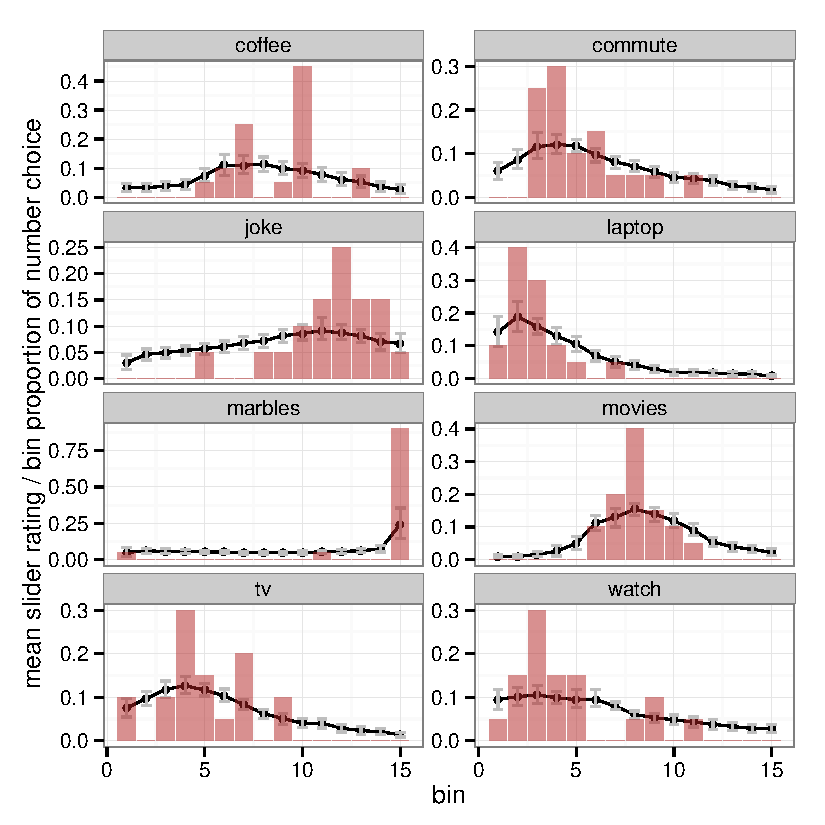
\includegraphics[width = \textwidth]{plots/data_sliderNumber.pdf}
    \caption{Red: proportion of bins corresponding to number choices on \emph{give-a-number} trials. Black: mean slider ratings on \emph{binned histogram} trials.}
    \label{fig:slider}
  \end{subfigure}

  \begin{subfigure}{0.475\textwidth}
    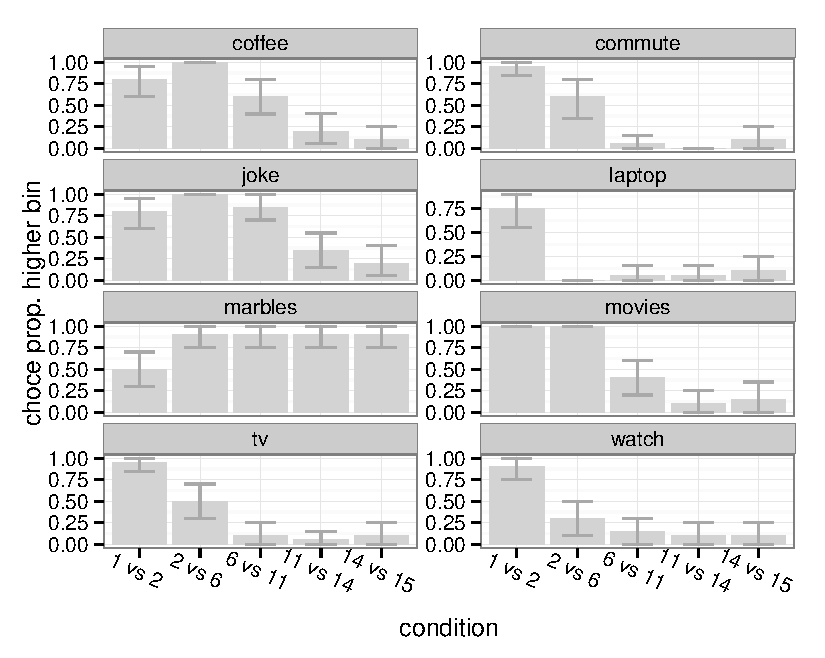
\includegraphics[width = \textwidth]{plots/data_choice.pdf}
    \caption{Proportion of higher bin choices on \emph{paired comparison} trials.}
    \label{fig:lighting}
  \end{subfigure}

  \caption{Average data. Bars are bootstrapped 95\% CIs.}
  \label{fig:Results}
\end{figure}

\section{Model}

The data we would like to explain are: (i) the normalized slider ratings $s_{ijk} \in [0;1]$ of
participant $i \in \set{1, \dots, 20}$ for item $j \in \set{1, \dots, 8}$ and bin
$k \in \set{1, \dots, 15}$ from the binned histogram task; (ii) the bins
$n_{ij} \in \set{1, \dots, 15}$ in which participant $i$'s number choice for item $j$ was in
the give-a-number task; and (iii) the binary choices $c_{ijl} \in \set{0,1}$ of whether
participant $i$ selected the higher bin for item $j$ in the paired comparison task for each
comparison $l$. There are two simplifications in need of commenting. In (i), we focus on slider
ratings after normalizing for each participant, because we assume that slider adjustments
reflect relative, not absolute estimates of subjective beliefs. In (ii), we focus on bin
choices, not actual number choices, in order to avoid, as much as possible, considerations of
salience of particular numbers, and also because otherwise data from items with smaller domains
of plausible numbers would get more weight than data from items with a wider range of
number choices. (Future work should investigate the relation to an explicit \emph{give-a-bin}
task.)

All three pieces of data are to be explained as functions of subjective beliefs $P_{ij}$, with
$P_{ijk}$ being participant $i$'s belief about the relative likelihood of bin $k$ for item
$j$. Each $P_{ij}$ defines a likelihood for our data, via appropriate link functions. Variance
in subjective beliefs is harnessed by a population-level hyper-prior with central tendency
$Q_{j}$. The structure of this model is pictured in \figref{fig:ModelGraph}.



To fill the structure in \figref{fig:ModelGraph} with life, we need to spell out three
parameterized link functions, one for each task type, and the relation between population-level
belief $Q_j$ and individual beliefs $P_{ij}$. Let's start with the latter. The idea is that
$P_{ij}$ are noise-perturbed variants scattered around $Q_j$, with some parameter $w$ to
determine how much perturbation we should expect.  To realize this, the model assumes that
$P_{ij}$ are distributed according to a Dirichlet distribution with weights given by $w Q_{j}$:
\begin{align*}
  Q_j & \sim \text{Dirichlet}(1, \dots, 1) & w & \sim \text{Gamma}(2,0.1) \\
  P_{ij} & \sim \text{Dirichlet}( w Q_j)
\end{align*}
The higher $w$, the more likely it is that $P_{ij}$ is ``close'' to $Q_j$.

The link function for the \textbf{slider rating data} uses a logit transformation to project observed
slider ratings $s_{ijk}$ and latent probabilities $P_{ijk}$, which are bound to lie between 0
and 1, to the reals. The likelihood of logit-transformed observation $s_{ijk}$ is given by a
Gaussian with standard deviation $\sigma$ around the logit-transformed predictor $P_{ijk}$. On
top of that, there is a parameter $\kappa$, the steepness of the logit transform of $P_{ijk}$,
that allows response likelihoods to capture end-point affinity for $\kappa >1$ (values of
$P_{ijk}$ close to 0 or 1 are likely mapped to 0 or 1) or end-point aversion for $\kappa <0$
(values of $P_{ijk}$ are likely to be realized as more median), with a prior that expects
$\kappa=1$.
\begin{align*}
  \text{logit}(s_{ijk}) &\sim
        \text{Norm}(\text{logit}(P_{ijk}, \kappa), \sigma) \\
        \sigma &  \sim \text{Gamma}(0.0001,0.0001) & \kappa &\sim \text{Gamma}(5,5)
\end{align*}
 
The link function for \textbf{number choice data} treats each bin $n_{ij}$ as a draw from a categorical
distribution where the probability of bin $k$ is proportional to $\expo(a P_{ij})$, i.e., a
soft-max choice from $P_{ij}$. The higher parameter $a$, the more likely $n_{ij}$ is the mode
of $P_{ij}$. For $a \rightarrow 0$, all bins become equiprobable.
\begin{align*}
  n_{ij} & \sim
        \text{Categorical}(\expo(a P_{ij})) &
 a & \sim \text{Gamma}(2,1)
\end{align*}

Finally, consider the link function for \textbf{bin comparisons}. We are interested in the
likelihood with which participant $i$ selects the higher bin for item $j$ in bin comparison
condition $l$. Suppose $l$ is about comparing the lower bin $b_l$ to the higher $b_h$. 
Perhaps the most natural approach would be to link the likelihood of choosing $b_h$ over $b_l$ to
the difference between $P_{ijb_h}$ and $P_{ijb_l}$. However, as discussed above, this does not
appear to be what participants were doing. Indeed, a model that implements this idea blatantly
fails to capture the relevant regularities in the data. Another plausible link function is to
assume that what matters is the distance to the mode of $P_{ij}$: soft-max prefer the bin that
is closer to the mode of $P_{ij}$; select randomly if both bins are equally far from the
prototype.\footnote{$(1 + \exp(2b(1-x)) )^{-1} = \frac{\exp(b x)}{\exp(b
    x) + \exp(b y)}$
  if $x = 2 - y$.}
\begin{align*}
  c_{ijl} & \sim \text{Bern}( (1 + \exp(2b(1-p^{\text{high}}_{ijl})) )^{-1} ) \ \ \ 
  b  \sim \text{Gamma}(2,1) \\
  p^\text{high}_{ijl} & = \begin{cases}
    2 & \text{if $mode(P_{ij})$ is closer to higher} \\
    & \text{ bin of $l$ than to lower bin } \\ 1 & \text{if equal
      distance} \\ 0 & \text{otherwise}  
  \end{cases}
\end{align*}

\begin{figure}[]
  \centering
  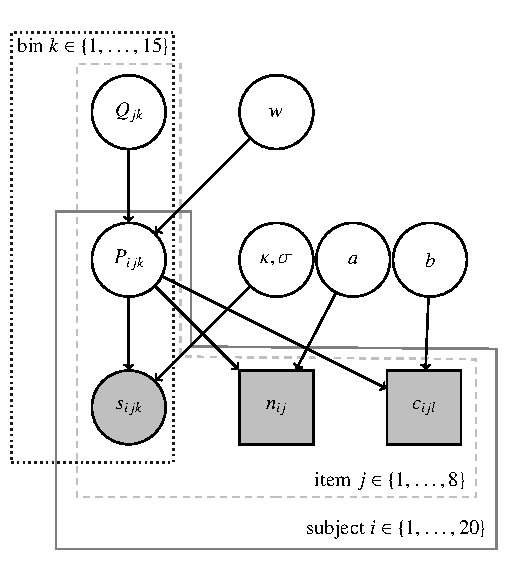
\includegraphics[width = 0.35\textwidth]{modelGraph/modelGraphNoMath.pdf}
  \caption{The data-generating model as a probabilistic graphical model, following conventions
    of \citet{LeeWagenmakers2013:Bayesian-Cognit}. Shaded nodes are observed, white nodes are
    latent variables. Square nodes represent categorical, round nodes continuous
    variables. Boxes indicate scope of indices.}
  \label{fig:ModelGraph}
\end{figure}

\section{Inference}

The model was implemented in JAGS \cite{Plummer2003:JAGS:-A-Program}. 50,000 samples were
obtained from two chains with a thinning rate of 2 after a burn-in of 100,000 that ensured
convergence according to $\hat{R}$ \cite{GelmanRubin1992:Inference-from-}.

Means and bounds of 95\% high-density intervals (HDIs) of the posteriors for model parameters are in
Table~\ref{tab:SummaryStats}. Posterior credible levels of $w$ allow for a limited amount of
slack around $Q_j$. Values for $\kappa$ indicate that, on average, participants had no
preference for or against extreme slider ratings. Relatively high values of $a$ indicate that
participants, on average, had a strong tendency to choose modal values in the \emph{give-a-number}
task.
\begin{table}[ht]
\centering
\footnotesize
\begin{tabular}{rlllll}
 & $w$ & $\kappa$ & $\sigma$ & $a$ & $b$ \\ \midrule
  lower & 14.65 &  0.98 &  0.26 & 22.04 &  1.11 \\ 
  mean & 15.55 &  0.99 &  0.28 & 27.43 &  1.27 \\ 
  upper & 16.48 &  0.99 &  0.31 & 32.95 &  1.42 \\ 
\end{tabular}
\caption{Summary statistics for posteriors on parameters}
\label{tab:SummaryStats}
\end{table}

Posterior estimates of $Q_j$ are the most relevant. \figref{fig:PosteriorQj} shows their means
with their 95\% HDIs, alongside the mean slider ratings. The latter provide a very good
approximation of the inferred population-level beliefs. Inspection of posteriors of
individual $P_{ij}$ shows that there is ample variation between participants. Still, the
way the model suggests we should think about harnessing the individual $P_{ij}$s under a
population-level central tendency is closely approximated by mean slider ratings. Although the
match is not perfect, it is good enough to say that the latter are a practical way of
approximating what the crowd believes despite individual differences.

\begin{figure}
  \centering
  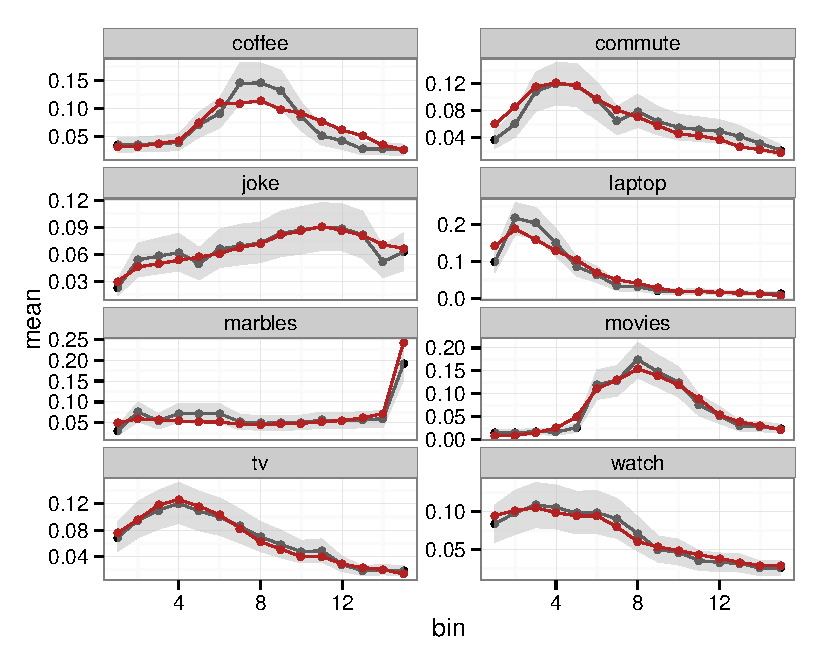
\includegraphics[width = 0.5\textwidth]{plots/pop_priors.pdf}
  \caption{Means of posteriors over $Q_j$ in black with gray area indicating 95\% HDIs. Red: mean slider ratings.}
  \label{fig:PosteriorQj}
\end{figure}

\section{Model criticism}

Inferences based on the model are only as reliable as the model itself is plausible. Model
criticism is therefore important. \figref{fig:PPCs} shows posterior predictive checks at the
population-aggregate level for all of our three task types. For the binned histogram task,
posterior predictions are spot-on. For the give-a-number task, some of the data is surprising
despite the model being trained on this very data. This could have various reasons: (i) the
give-a-number data does not have a huge influence on the posterior likelihood, (ii) number
choices may be influenced by saliency and/or roundness of numbers after all (and thus, not
accurately reflect the true beliefs $Q_j$). Finally, there is one condition in the paired
comparison task that the model definitely got wrong. This is the choice of what is more likely:
that one or that none of 14 marbles thrown into a pool would sink. The model predicts that
almost everybody should answer that it is more likely that one marble sank. But that is not
what we observe. It may be that participants revise beliefs about ``normality'' of the marbles,
while holding on to an assumption that all marbles behave in the same way
\cite{DegenTessler2015:Wonky-worlds:-L}.

\begin{figure}
  \centering
  \begin{subfigure}[b]{0.5\textwidth}
    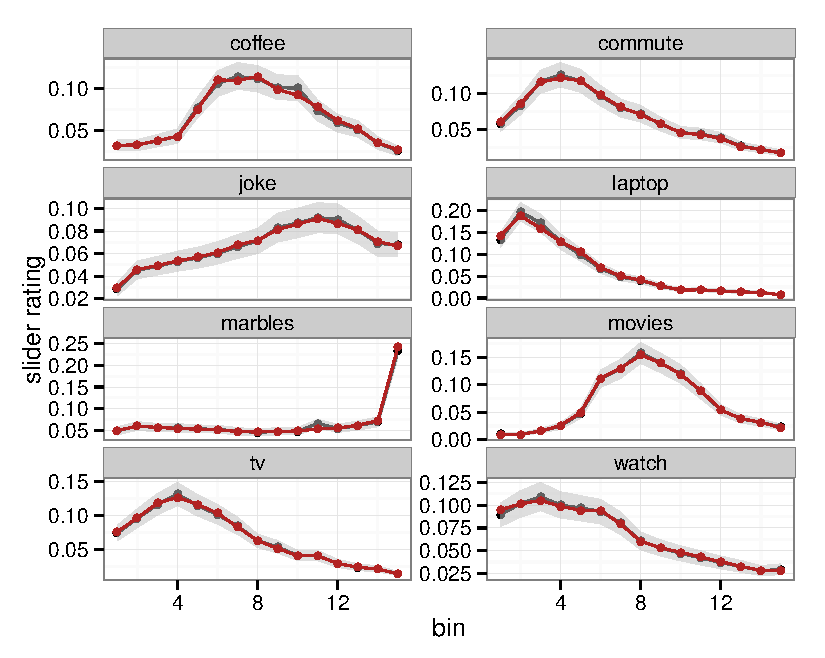
\includegraphics[width = \textwidth]{plots/ppc_slider.pdf}
    \caption{Binned histogram task.}
    \label{fig:sliderPPC}
  \end{subfigure}
   
  \begin{subfigure}[b]{0.5\textwidth}
    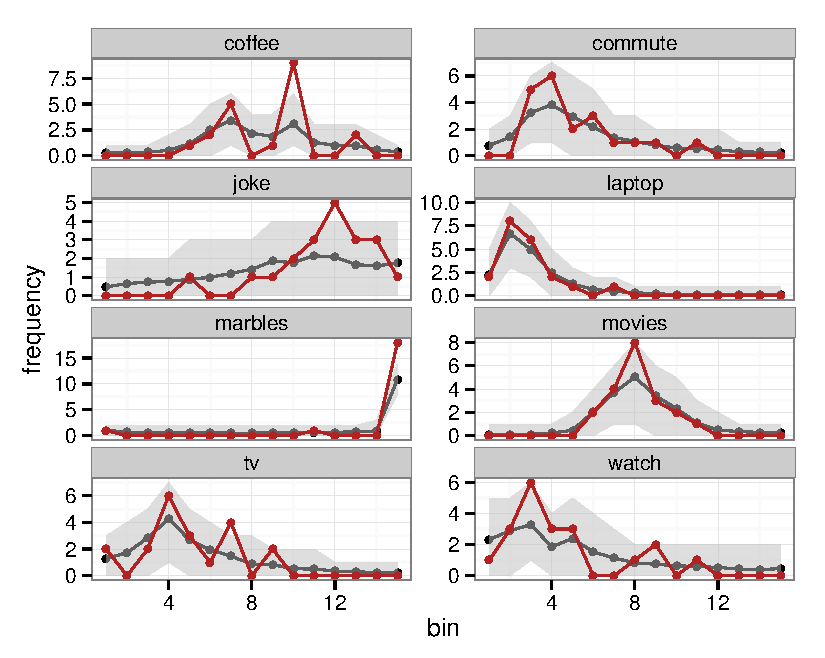
\includegraphics[width = \textwidth]{plots/ppc_number.pdf}
    \caption{Give-a-number task.}
    \label{fig:numberPPC}
  \end{subfigure}

  \begin{subfigure}[b]{0.5\textwidth}
    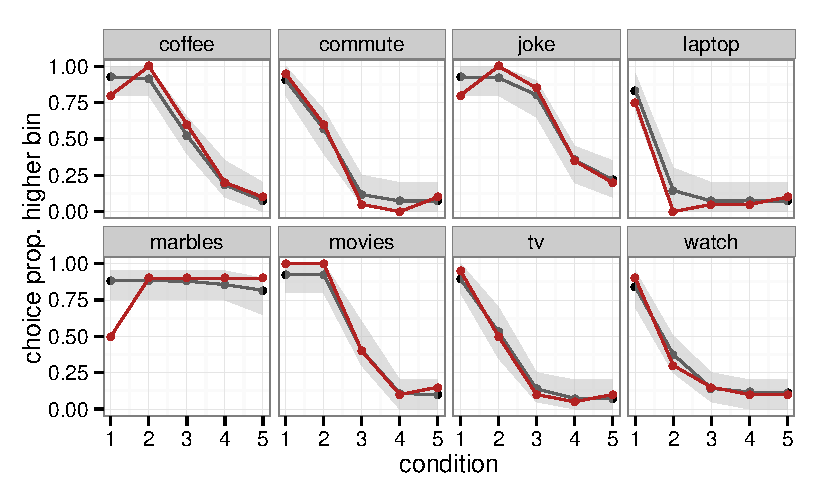
\includegraphics[width = \textwidth]{plots/ppc_choice.pdf}
    \caption{Paired comparison task.}
    \label{fig:lightingPPC}
  \end{subfigure}

  \caption{Posterior predictive checks for aggregate data. Red lines give empirical
    observations. Black lines are means of posterior predictive samples, gray areas are
    95\% HDIs.}
  \label{fig:PPCs}
\end{figure}

Posterior predictive checks indicate that the trained model captures patterns of answers at the
aggregate population level well. To have a more fine-grained measure of model fit, we also
looked at posterior predictive $p$-values \citep{GelmanCarlin2014:Bayesian-Data-A} at the level
of participants and items. We look at the binned histograms task, because this is our main
focus here and population-level posterior predictive checks for BH revealed no systematic
deviance. Fixing a participant and an item, observations and replicates are probability vectors
of length 15. In a first analysis, we used the mean of these probability vectors as a test
statistic. The minimum posterior predictive $p$-value over all 20 (participants) times 8
(items) cases was 0.13, suggesting that the means of observed $s_{ij}$ are non-surprising to
the trained model. In a second analysis, we used entropy as a test statistic. Two cases gave
posterior predictive $p$-values lower than 0.05. These were from the two participants who gave
a very extreme slider rating for the ``marbles'' item, basically assigning all ``mass'' to the
last bin. What this suggests is that the model can cope reasonably well also with
individual-level data, but, somewhat unsurprisingly, has problems accounting for ``extreme''
choices, given that the population-level hyper-prior on $P_{ij}$ will lead to shrinkage.

\section{Conclusion}

The data and model presented here suggest that mean slider ratings are consistent with other
measures of subjective belief, namely from give-a-number and paired comparison tasks. Future
research should evaluate whether this holds for other possible measures of subjective beliefs
as well, such as iterated-learning or scoring-rule tasks. 

There are aspects of the data that the model does not capture well, but there are also natural
explanations for these discrepancies. It therefore does not seem implausible that participants'
latent beliefs could have generated the data from all three task types roughly in the way
assumed by the model's link functions, with each subjective belief being an expression of a
population-level central tendency. If that is so, then mean slider ratings from the binned
histogram task are a practical and reliable approximation of what the crowd believes.

Future research should investigate whether and how our results can be extended to other types
of uncertain variables. Here, guided by the needs of many previous Bayesian cognitive models,
we focused on uncertainty about unidimensional contiguous variables. It remains to be seen
whether the binned histogram task can be applied to higher-dimensional variables, like joint
prior beliefs over, say, \emph{height} and \emph{weight} of an individual or, more abstractly,
different dimensions of a multi-dimensional property like \emph{intelligence}. Another
challenge lies in devising means of eliciting prior expectations about properties that do not
have clear and familiar measure terms that can be used to label bins---again like \emph{intelligence}.

Finally, another aspect that our model has ignored so far are potential individual differences
in the way subjective beliefs $P_{ij}$ generate responses. It is not unlikely that there is
individual variation in at least some link function parameters, such as $\kappa$, which
expresses end-point attraction or end-point aversion in the binned histograms task. A detailed
investigation of such individual-level differences must be left to future work. Still, we
believe that the model presented here is an important first step towards finding reliable and
practical means of measuring what the crowd believes.

\section{Acknowledgments}

MF's work was supported by the Institutional Strategy of the University of T̈\"{u}bingen
(DFG, ZUK 63). MF, FD, AS and JD's work was supported by the
Priority Program XPrag.de (DFG Schwerpunktprogramm 1727). This work was further supported by
ONR grant N00014-13-1-0788 and a James S. McDonnell Foundation Scholar Award to NDG and an SNF
Early Postdoc.Mobility Award to JD. Thanks to three anonymous reviewers for helpful suggestions
and criticism.



\bibliographystyle{apacite}

\setlength{\bibleftmargin}{.125in}
\setlength{\bibindent}{-\bibleftmargin}

\bibliography{references}


\end{document}
